
\chapter{Petit Fourier}

A \emph{petit four} is a small dessert that translates to \emph{small oven} in French. In this chapter we explore Fourier series and Fourier transforms: a way to write functions of space with respect to a \emph{basis} of oscillating functions. This paves the way to Chapter~\ref{ch:function:space} where we properly examine the space of functions as a metric space.

In this chapter $n$ and $m$ are understood to be integers that we use to index basis functions. They replace $i$ and $j$ to avoid confusion with $i=\sqrt{-1}$. 

\section{Asymmetric Interval}

As a starting point, consider the interval $0 \leq x \leq L$. A common problem in first year physics is to ask for the kinds of functions $f(x)$ that could exist on this interval while satisfying $f(0)=f(L)=0$. These are called \textbf{Dirichlet boundary conditions}. 
\begin{example}
The function $f(x)=x$ satisfies $f(0)=0$, but does \emph{not} satisfy $f(L)=0$. 
\end{example}
The functions that satisfy this are probably familiar from your coursework on waves:
\begin{align}
    s_n(x) \defeq A_n \sin(k_n x) \ ,
\end{align}
where $A_n$ is some normalization. We remember that $\sin 0 = 0$ so all the functions satisfy $s_n(0)=0$. What about the boundary condition at $L$? We cannot set $A_n$ to zero since that would make $f_n(x) = 0$ for all $x$. All we are left with is a choice for $k_n$. There is an entire family of $k_n$ choices that satisfies $s_n(L)=0$; indeed, this is why we introduce the label $n$:
\begin{align}
    k_n = \frac{n\pi}{L} \ .
\end{align}
\begin{exercise}
Show that $\sin(k_n L) = 0$ for any integer $n$. 
\end{exercise}

Observe that linear combinations of the $f_n(x)$ functions also satisfy the boundary conditions:
\begin{align}
    g(x) = c^n s_n(x) = c^1 s_1(x) + c^2 s_2(x) + \cdots. 
\end{align}
This is true because at $x=0$ and $x=L$, each term in the sum vanishes. At this point, you recognize from our notation that this resembles a vector space where \emph{the vectors are functions}. We may write
\begin{align}
    \ket{g} = c^n \ket{s_n} \ ,
\end{align}
where $\ket{s_n} =A_n \sin k_n x$ is a \emph{basis} for this \emph{function space}. 
\begin{exercise}
The sum over $n$ is formally infinite. It runs form $n=1$ to $n=\infty$. Why is it not necessary to include negative values of $n$? \textsc{Hint:} In fact, it would be inappropriate to do this because those functions are redundant.
\end{exercise}

There is an inner product for this function space:
\begin{align}
    \la g, h \ra = \int_0^L \D{x}\, g(x)^* h(x) \ .
\end{align}
Because all of our functions and coefficients are real, one may ignore the complex conjugation.\sidenote{We write it out explicitly so that you get used to seeing it there.}
\begin{exercise}
Show that with this inner product, the proper normalization for the basis functions $\ket{f_n}$ is
\begin{align}
    A_n = \sqrt{\frac{2}{L}} \ .
\end{align}
\textsc{Remark}: You could have guessed the $L$ dependence form dimensional analysis.\sidenotemark
\end{exercise}\sidenotetext{There is also a clever way to calculate the 2. To do thus, use $\sin^2\theta + \cos^2\theta =1$ and then integrate over half of a period. Argue that both terms contribute equally.}

The result is a Fourier sine series: a space of functions that are linear combinations of the form $c^n\ket{s_n}$.  What about other functions? You could imagine, for example, the function 
\begin{align}
    g(x) = \left(x-\frac{L}{2}\right)^2 - \left(\frac{L}{2}\right)^2
\end{align}
satisfies the boundary conditions and clearly is not in the form of a sine. If $\ket{f_n}$ is to be a basis for all functions satisfying the boundary conditions, how can we see that $g(x)$ may be expressed as a sum over basis functions? We need
\begin{align}
    g(x) = \ket{g} = g^n\ket{s_n} \ .
\end{align}
Fortunately, we know how to write the components of a vector. Recall that $v^i = \la e^i \mid v \ra = \la e_i, v \ra$. Using our function space inner product,
\begin{align}
    g^n = \la s_n, g \ra 
    = \int_0^L \D{x}\, A_n \sin(k_n x) \, g(x)  \ .
\end{align}
By performing this integral for any positive integer $n$, you may identify the coefficients $g^n$.
\begin{exercise}
Calculate the first few components, $g^1$, $g^2$, and $g^3$. Argue that it should be obvious in hindsight that $g^2 = 0$. \textsc{Hint:} plot the functions $g(x)$ and $s_n(x)$ and think about symmetries of the integrand.
\end{exercise}




\section{Other boundary conditions}

There are three common types of boundary conditions at a boundary, $a$:
\begin{enumerate}
    \item \textbf{Dirichlet}: the function vanishes, $f(a)=0$.
    \item \textbf{Neumann}: the derivative of the function vanishes, $f'(a)=0$. 
\end{enumerate}
An interval in one dimension has two boundaries, say $a \leq x \leq b$. You may have any mixture of the above two boundary conditions:
\begin{align}
    \text{Dirichlet--Dirichlet:}
    &&
    f(a)&=f(b)=0
    \\
    \text{Neumann--Neumann:}
    &&
    f'(a)&=f'(b)=0
    \\
    \text{Dirichlet--Neumann:}
    &&
    f(a)&=f'(b)=0
    \\
    \text{Neumann--Dirichlet:}
    &&
    f'(a)&=f(b)=0
    \ .
\end{align}
A third type of boundary condition is:
\begin{enumerate}
    \item[3] \textbf{Periodic}: $f(a)=f(b)$ and $f'(a)=f'(b)$. This is the boundary condition you expect if the interval $a\leq x \leq b$ is wrapped around a circle with $a$ and $b$ identified. For example, $a=0$ and $b=2 \pi$. 
\end{enumerate}


\paragraph{Why are always two boundary conditions?} Observe that the boundary conditions always come in pairs. This is because you need two boundary conditions to specify a function. This, in turn, is because we almost always work with second order differential equations.\sidenote{These are always some form of the Laplacian and always contain two derivatives.} \emph{This}, in turn, is because the dynamics in physics are described by \emph{local} dynamics, see \bigidearef{}~\ref{idea:causality:and:derivatives}. Equations that carry higher derivatives are typically subleading.

\paragraph{What goes wrong with other boundary conditions?}
% 
What if you want to impose another boundary condition? It turns out that it is remarkably difficult to impose other boundary conditions that lend themselves to the \emph{vector space structure} that we wish to utilize in our space of functions.

\begin{example}
Consider the interval $0\leq x \leq L$ with the boundary conditions $f(0)=0$ and $f(L)=a$, where $a\neq 0$ is some constant. Consider two functions that satisfy this:
\begin{align}
    g(x) &= \frac{ax}{L}
    &
    h(x) &= \frac{ax^2}{L^2} \ .
\end{align}
It is clear that the sum of these functions $g(x)+h(x)$ does \emph{not} satisfy the boundary condition $f(L)=0$. In fact, most linear combinations of $g(x)$ and $h(x)$ do not satisfy this second boundary condition.
\end{example}
\begin{exercise}
Prove that linear combinations of functions with Dirichlet and/or Neumann boundary conditions still satisfy those boundary conditions. Prove that linear combinations of functions with periodic boundary conditions still satisfy the periodic boundary conditions.
\end{exercise}

\paragraph{What if the interval becomes infinite?}
A common scenario in physics is that the boundary is infinitely far away. Then you may wonder what boundary condition you should apply. Maybe you wonder if it even matters?

Sometimes it matters. For example, if the function you are considering represents a physical quantity that carries some energy density, then it may be problematic to have a boundary condition where that density does not go to zero at infinity. Usually we say that functions must die off sufficiently quickly at infinity---where the phrase \emph{sufficiently quickly} depends the nature of the problem.\sidenote{What we usually mean is that the physics at infinity should not affect the physics \emph{here}.} Sometimes we know that the behavior at infinity simply does not matter and thus we may pick periodic boundary conditions because they are numerically well behaved.\sidenote{Periodic boundary conditions correspond to \emph{no boundary} and prevent any ``edge effects'' when running a large simulation.}

\section{Parallel Plate Example}

Consider the electrostatics problem shown in Figure~\ref{fig:griffiths:3:17} from Griffiths' \emph{Introduction to Electrodynamics}.
\begin{marginfigure}
    \centering
    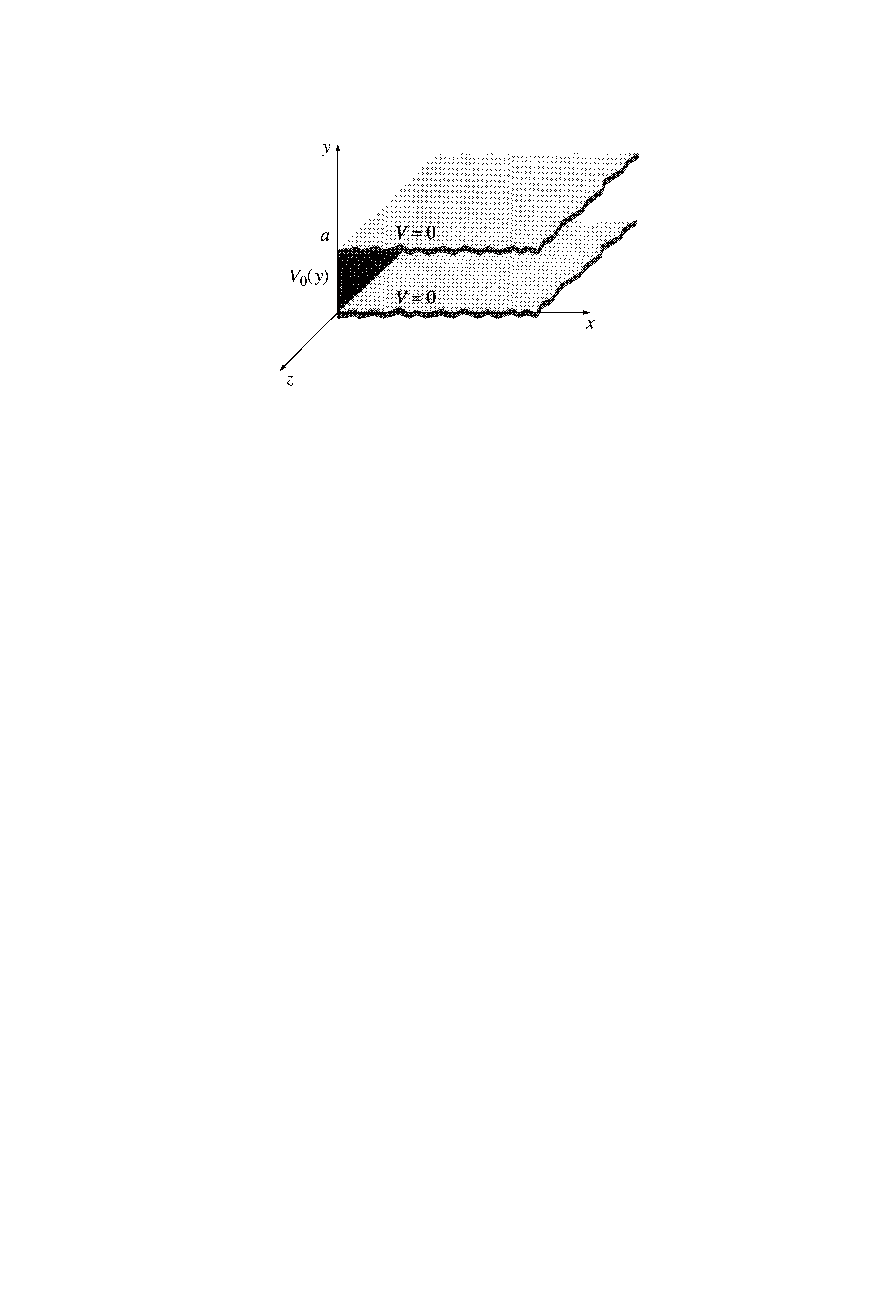
\includegraphics[width=\textwidth]{figures/GriffithsEM3_17.pdf}
    \caption{Two infinite grounded metal plates are parallel on the $xz$ planes, separated by a distance $a$ in the $y$ direction. There is an infinite strip at $x=0$ that is insulated from the grounded plates and is fixed to obey a potential $V_0(y)$. Fig.~3.17 in Griffiths, \emph{Introduction to Electrodynamics}.}
    \label{fig:griffiths:3:17}
\end{marginfigure}
The problem is to solve for the electrostatic potential $V(x,y,z)$ in the region inside the plate configuration, $x>0$ and $0<y<a$.

Because the problem has no $z$-dependence, the solution must be independent of $z$. We thus have $V=V(x,y)$. This means that $\partial_z^2 V = 0$ and the potential satisfies a simplified Poisson equation,
\begin{align}
    \nabla^2 V(x,y) = 
    \frac{\partial^2V}{\partial x^2}
    +
    \frac{\partial^2V}{\partial y^2}
    = 0 \ .
    \label{eq:2d:Poisson:eg}
\end{align}

It is now typical to make a \emph{guess}\sidenote{To the best of my knowledge this is really a guess based on knowing that this guess often works in physics. There may be some mathematical argument why the Laplacian always admits separable solutions. It is not obvious to me.} that the solution is \textbf{separable}:
\begin{align}
    V(x,y) \stackrel{?}{=} X(x) \, Y(y)
    \ .
    \label{eq:separation:2d:eg}
\end{align}
If we take this assumption, we find that
\begin{align}
    \frac{X''(x)}{X(x)} + \frac{Y''(y)}{Y(y)} = 0 \ .
    \label{eq:separation:too:eg}
\end{align}
\begin{exercise}
Show that \eqref{eq:separation:too:eg} follows from plugging \eqref{eq:separation:2d:eg} into \eqref{eq:2d:Poisson:eg} and then dividing everything by $V(x,y)$.
\end{exercise}
Because the first term of \eqref{eq:separation:too:eg}  only depends on $x$ and the second term only depends on $y$, we find that each term must be constant with equal magnitude and opposite sign. We thus write
\begin{align}
    X'' &= k^2X & Y''&= -k^2 Y \ .
    \label{eq:two:equations}
\end{align}
Observe that it is the \emph{same} $k^2$ for each equation.
% 
Note that we have made a choice here and have written the coefficient of the $Y$ equation to be \emph{negative} while the coefficient of the $X$ equation is \emph{positive}. This is also physically motivated, as we shall see shortly.

Assuming that $k^2>0$, the general solutions to the $X$ equation are
\begin{align}
    X(x) &= Ae^{kx} + Be^{-kx} \ ,
\end{align}
for some constants $A$ and $B$. Physically, we know that $X(x\to\infty)$ should go to zero because one is arbitrarily far from the charge distribution producing $V_0(y)$. This is an \emph{implicit} boundary condition that was not stated in the problem, but that we should know from ``physical sensibility.'' We thus recognize that $A=0$.

\begin{example}
If $A\neq$ then for arbitrarily large $x\gg 1$ you would find arbitrarily an arbitrarily large electric field $E\sim Ake^{kx}$. This would be very physically implausible as there is nothing to  source this huge electric field.
\end{example}

\begin{exercise}\label{ex:two:equations:wrong:choice}
Why should we have guessed that \eqref{eq:two:equations} had the correct sign assignment between the $X$ and $Y$ equations? Check what happens if you swap the signs:
\begin{align}
    X'' &= -\bar k^2X 
    & Y''&= \bar k^2 Y \ .
    \label{eq:two:equations:wrong}
\end{align}
What is the apparent contradiction that we find relative to the $X(x\to\infty)$ boundary condition? If you stare at the contradiction long enough, you may find a clever way out where you allow $\bar k=ik$ to be a purely imaginary number---but at that point you simply recover \eqref{eq:two:equations}. 
\end{exercise}

The $Y(y)$ equation in \eqref{eq:two:equations} and the boundary conditions $Y(0)= Y(a) = 0$ are precisely what we expect from our basis of sines on the interval $0 \leq x \leq a$, $\ket{s_n} = (2/a)^{1/2}\sin (n\pi y/a)$. This means that \emph{any} linear combination of the basis functions $\ket{s_n}$ satisfies the $Y$ equation. Each one of these has their own value of $k_n$:
\begin{align}
    \partial_y^2 \ket{s_n} = -\left(\frac{n\pi}{a}\right)^2 \ .
\end{align}

This means that our separation of variables guess \eqref{eq:separation:2d:eg} should be written as a sum:
\begin{align}
    V(x,y) = \sum_n e^{-k_n x} \; v^n \sqrt{\frac{2}{a}} \sin \frac{n\pi y}{a} \ ,
    \label{eq:general:Vxy:eg}
\end{align}
where $v^n$ are the components of $\ket{Y} = v^n\ket{s_n}$. We have absorbed the overall coefficient $A$ into the to-be-determined components $v^n$. We have attached the $e^{-k_nx}$ term from the $X(x)$ equation because it is the \emph{same} $k_n = (n\pi/a)$ that shows up in the $Y(y)$ equation---see \eqref{eq:two:equations}.

The general solution \eqref{eq:general:Vxy:eg} satisfies the Poisson equation \eqref{eq:2d:Poisson:eg}, but we need the specific set of coefficients $v^n$ that reproduce the boundary condition $V(x=0,y) = V_0(y)$ for some function $V_0(y)$ that satisfies $V_0(0) = V_0(a) = 0$. Clearly $V_0(y)$ is a function in our function space, $\ket{V_0} = u^n \ket{s_n}$. Setting $\ket{V} = \ket{V_0}$ at $x=0$ then gives (using $e^-0 = 1$) \ .
\begin{align}
    v^n \ket{s_n} = u^n \ket{s_n}
\end{align}
Thus for any $V_0(y)$ satisfying the boundary conditions, we may find the Fourier components $u^n$ and equate $v^n = u^n$.


\section{Functions on the circle}

We write the circle as $S^1$, which means the one-dimensional sphere. It is an interval $\theta \in [-\pi, \pi]$ where the points $\theta = \pi$ and $\theta = -\pi$ are identified.\sidenote{It is obvious that you could equivalently define this over the interval $\theta\in[0,2\pi]$ with $0$ and $2\pi$ identified.} This identification is a boundary condition. In this section we consider functions $f(\theta)$ that map points on the circle to numbers. The boundary condition is simply that $f(-\theta) = f(\theta)$. In fact, we may write the boundary condition a bit more cleanly:
\begin{align}
    f(\theta) = f(\theta+2\pi) 
    \label{eq:periodic:boundary:conditions}
    \ .
\end{align}
This boundary condition allows us to `unwind' and extend the interval $\theta \in [-\pi, \pi]$ into the entire real line $\theta \in \mathbbm{R}$ with the understanding that you end up wrapping around the circle multiple times.\sidenote{This leads to the notion of a winding number: the number $\theta = 4\pi \equiv 0$ has wrapped around the circle twice to return to the origin. Sometimes---especially when you are integrating---a physical system keeps track of how many times you've gone around the circle.}
% 
This boundary conditions is precisely the \textbf{periodic boundary condition} we identified above.  
\flip{Comment on this being a quotient space. I think Penrose had a nice way of saying this in \emph{Road to Reality}.}
% 
If you are a stickler for differential equations, you might argue that \eqref{eq:periodic:boundary:conditions} is just \emph{one} boundary condition but the function spaces in physics typically have \emph{two} boundary conditions because we want to solve second-order differential equations. You can check that \eqref{eq:periodic:boundary:conditions} simultaneously implies $f'(\theta) = f'(\theta + 2\pi)$.

\begin{exercise}
Use the definition of the derivative to show that \eqref{eq:periodic:boundary:conditions} actually implies an infinite number of boundary conditions: $f^{(n)}(\theta) = f^{(n)}(\theta+ 2\pi)$ where $f^{(n)}$ is the $n^\textnormal{th}$ derivative of $f(\theta)$. 
\end{exercise}

The trigonometric functions are simply the $x$ and $y$ coordinates of points on the unit circle. They \emph{tautologically}\sidenote{To quote Tony Zee, this means \emph{more obvious than obvious}. But the word `tautologically' says it in a way that sounds mathematical and refined.} satisfy the periodic boundary condition \eqref{eq:periodic:boundary:conditions}. 


\subsection{Averaging over a period}

Sine and cosine turn out to have some nice properties when you average them over the circle.  
%
Let us start with a simple statement. The average of sine or cosine over an entire period vanishes:
\begin{align}
    \frac{1}{2\pi}
    \int_{-\pi}^\pi d\theta\, \sin n\theta 
    &= 0
    \\
    \frac{1}{2\pi}
    \int_{-\pi}^\pi d\theta\, \cos n\theta 
    &= 0
    \ .
\end{align}
If you draw a plot of sine and cosine it is clear that the positive parts and negative parts cancel each other out when summing over the period.

What if we square the functions? The average over the \emph{square} of the trigonometric functions is one half:
\begin{align}
    \frac{1}{2\pi}
    \int_{-\pi}^\pi d\theta\, \sin^2 n\theta 
    % &= \frac{1}{2}
    % \\
    =
    \frac{1}{2\pi}
    \int_{-\pi}^\pi d\theta\, \cos^2 n\theta 
    &= \frac{1}{2} 
    &
    n
    &> 0
    \ .
    \label{eq:average:of:square:of:trig}
\end{align}
This should catch your eye as a linear algebraist because it looks \emph{a lot} like the the normalization condition for a basis vector in a function space. 

\begin{exercise}
Prove the conditions \eqref{eq:average:of:square:of:trig}. There is a clever way to do this. Start with the usual trigonometric identity
\begin{align}
    \sin^2\theta + \cos^2\theta = 1 \ .
\end{align}
Integrate both sides over an entire period in $\theta$. Then argue that the sine and cosine integrals are equivalent because they only differ by a phase. The relative phase between sine and cosine is irrelevant when integrating over the entire period. 
\end{exercise}


The average over the sine times the cosine vanishes:
\begin{align}
    \frac{1}{2\pi}
    \int_{-\pi}^\pi d\theta\, \sin n\theta \, \cos m\theta 
    &= 0 \ .
    \label{eq:fourier:trig:cos:sin}
\end{align}
\sidenotetext{When I say `prove' you can read this as ``make a convincing case to a physicist.''}
\begin{exercise}
Prove\sidenotemark \eqref{eq:fourier:trig:cos:sin} for any integers $n$ and $m$. \textsc{Hint}: draw a picture of the sine and cosine functions for small values of $n$ and $m$. In fact, you may want to start with $m=0$ and $n=1,2,3$. Argue that every positive contribution in the integral is canceled by an equal negative contribution. Then see what happens when $m=1$. After some thought (and plotting if needed), convince yourself that the fact that sine is odd and cosine is even guaranteees that the integral over an entire period \eqref{eq:fourier:trig:cos:sin} vanishes.
\end{exercise}
The average over two of the same trigonometric function but with different integers scaling the argument also vanishes:
\begin{align}
    \frac{1}{2\pi}
    \int_{-\pi}^\pi d\theta\, \sin n\theta \,\sin m\theta 
    &= 0
    &
    \text{if }n\neq m&
    \\
    \frac{1}{2\pi}
    \int_{-\pi}^\pi d\theta\, \cos n\theta \,\cos m\theta 
    &= 0 
    &
    \text{if }n\neq m&
    \ .
\end{align}
\begin{exercise}
Prove these `orthogonality' relations. \textsc{Hint}: like the previous exercise, it helps to plot $\sin n\theta$ and $\sin m\theta$ on the same graph for some choice of $n\neq m$. Check that every region where the product takes some value is paired with another region where the product is negative that value.
\end{exercise}


Now take a deep breath and look at these `average over a period' relations. 
Taken together, they look remarkably like orthogonality conditions. Let us propose the following basis for the function space $S^1$:
\begin{align}
    \ket{s_n} &= \sqrt{\frac{1}{\pi}} \sin n\theta
    &
    n&>0
    \label{eq:foruier:S1:sine:basis}
    \\
    \ket{c_n} &= \sqrt{\frac{1}{\pi}} \cos n\theta 
    &
    n&> 0
    \label{eq:foruier:S1:cosine:basis}
    \\
    \ket{c_0} &= \sqrt{\frac{1}{2\pi}} 
    \label{eq:foruier:S1:cosine:zero:basis}
    \ .
\end{align}
The basis function $\ket{c_0}$ is simply a constant and needs to be treated differently.
\begin{exercise}
It may seem puzzling that $\ket{c_0}$ is not defined to be $\pi^{-1/2}\cos 0\theta$. Explain why \eqref{eq:foruier:S1:cosine:zero:basis} has a different normalization than \eqref{eq:foruier:S1:cosine:basis}. Confirm that \eqref{eq:foruier:S1:cosine:zero:basis} is a properly normalized basis function that represents constant functions on the circle, then explain why \eqref{eq:foruier:S1:cosine:basis} has a different normalization.  \textsc{Hint}: the origin of the normalization condition was \eqref{eq:average:of:square:of:trig}, which only holds for $n>0$.
\end{exercise}
\begin{exercise}
Show that $\ket{s_n}$ and $\ket{c_n}$ are orthonormal basis functions on the space of functions defined on the circle.
\end{exercise}



\subsection{An orthogonal set of functions}

Let $f(\theta)$ be a function over the circle $S^1$. This simply means that $f(\theta)$ is periodic with $f(\theta+2\pi) \equiv f(\theta)$. The crux of \textbf{Fourier series}\index{Fourier series} is that we may write this function as
\begin{align}
    f(\theta) 
    &= a^n\ket{c_n}
    + 
    b^n \ket{s_n}
    \\
    &= 
    % \frac{1}{2}a_0
    % + 
    \frac{a^0}{\sqrt{2\pi}}
    +
    \sum_{n=1}^\infty a^n \frac{\cos n\theta}{\sqrt{\pi}}
    + \sum_{m=1}^\infty b^m \frac{\sin m\theta}{\sqrt{\pi}} \ .
    \label{eq:fourier:series:sine:cos}
\end{align}
% We justify the convenient factor of half on the $a_0$ below. 
It is clear that each term in the above infinite sum is periodic and therefore the function is periodic.
\begin{exercise}[Completeness?] 
At this point you should wonder if \emph{any} periodic function $f(\theta)$ may be written in the above form. Alternatively, is there a unique map between periodic functions and the coefficients $a_{0,n}$ and $b_m$ for $n,m>0$? 

If you are mathematically inclined, you may prove the uniqueness this in some fancy way. As a physicist, convince yourself that you can clearly \emph{approximate} the behavior of any nice periodic function with a small number of coefficients with $n$ and $m$ close to zero. Make plots if you are uncertain. There's physical intuition here: the values of $n$ and $m$ correspond to wave numbers, or \emph{momenta}. What you observe here is that low wave numbers (small momenta) corresponds to large wavelengths, or long-distance features. This inverse relationship between momentum and distance is the crux of Heisenberg's uncertainty principle. It is also the reason why high-energy colliders are used to probe subatomic length scales.
\end{exercise}

Given a periodic function $f(\theta)$, how do you determine the \textbf{Fourier coefficients}\index{Fourier coefficient} $a^{n}$, $b^m$? We may simply use the inner product analog of $v^i = \la e_i, v\ra$:
\begin{align}
    a^n &= 
    \la c_n, f\ra =
    \begin{cases}
    \displaystyle
    \frac{1}{\sqrt{2\pi}}\int_{-\pi}^\pi
    \D{\theta}\, f(\theta) & n= 0
    \\
    \displaystyle
    \frac{1}{\sqrt{\pi}}\int_{-\pi}^\pi
    \D{\theta}\, f(\theta) \cos(n\theta) & n> 0
    \end{cases}    
    \\
    b^m &= 
    \la s_n, f\ra =
    \frac{1}{\sqrt{\pi}}
    \int_{-\pi}^\pi
    \D{\theta}\, f(\theta) \sin(m\theta) 
    & m&> 0
    \ .
\end{align}
% \begin{exercise}
% Prove these relations using the orthogonality relations in the previous subsection. You should not have to do any calculations other than a \emph{trivail} bit of algebra to confirm the factors of $\pi$ in the normalization. Note this justifies the factor of half on the $a_0$ coefficient: it is a convenient way write the constant term in terms of an overlap integral with $\cos n\theta$ for $n=0$.
% \end{exercise}
\begin{exercise}
Why is there no $m=0$ term? 
\end{exercise}

\begin{exercise}
Sometimes the Fourier series is introduced without any reference to basis functions or inner products---instead, one simply notes that certain integrals over two trigonometric functions vanish. Those discussions usually write the Fourier series in terms of the trigonometric functions rather than their normalized versions:
\begin{align}
    f(\theta) = \frac{1}{2}a_0
    + \sum_{n=1}^\infty a_n \cos n\theta
    + \sum_{m=1}^\infty b_m \sin m\theta \ .
    \label{eq:fourier:series:sine:cos:nonorm}
\end{align}
instead of \eqref{eq:fourier:series:sine:cos}. Show that with this strange normalization the Fourier coefficients are
\begin{align}
    a_n &= \frac{1}{\pi}\int_{-\pi}^\pi
    \D{\theta}\, f(\theta) \cos(n\theta) & n&\geq 0
    \\
    b_m &= \frac{1}{\pi}\int_{-\pi}^\pi
    \D{\theta}\, f(\theta) \sin(m\theta) 
    & m&> 0
    \ .
\end{align} 
Explain the factor of half on the $a_0$ term.
\end{exercise}

\subsection{Complex basis}
Trigonometric functions become easy when we write them in terms of complex exponentials:
\begin{align}
    e^{i\theta} = \cos\theta + i \sin\theta \ .
\end{align}
Inverting this gives
\begin{align}
    \cos\theta &= \frac{e^{i\theta} + e^{-i\theta}}{2}
    \\
    \sin\theta &= \frac{e^{i\theta} - e^{-i\theta}}{2i} 
    \ .
\end{align}
By plugging these into the trigonometric Fourier expansion \eqref{eq:fourier:series:sine:cos} we see that we may equivalently write any real periodic function $f(\theta)$ as
\begin{align}
    f(\theta) &= \sum_{n=-\infty}^\infty
    c_n e^{in\theta} \ ,
    \label{eq:fourier:complex:series}
\end{align}
where we observe that the integer index $n$ now takes on both positive and negative (and zero) values. 
\begin{exercise}
Express the coefficients $c_n$ in terms of the coefficients $a_n$ and $b_n$ in  \eqref{eq:fourier:series:sine:cos}.
\end{exercise}

You should be quick to say that $e^{in\theta}$ is not obviously orthonormal.
It is easy to see the orthogonality of the complex exponentials. For any integer $k\neq 0$, we see that
\begin{align}
    \int_{-\pi}^\pi \D{\theta} \, e^{ik\theta}
    = \frac{1}{ik}
    \left(e^{ik\pi} - e^{-ik\pi}\right) = 0 \ .
\end{align}
\begin{exercise}
Prove the above relation. One way to do this is to note that $e^{ik\pi} = e^{-ik\pi}$  for integer $k$, which you can see by plotting these points on the complex plane. Alternatively, one may write $e^{\pm i k\pi}$ in terms of cosine and sine functions and remember that $\cos(-\theta) = \cos \theta$ while $\sin(-\theta) = -\sin\theta$.
\end{exercise}
When $k=0$ the integrand is simply one and evaluates to $2\pi$. We thus have:
\begin{align}
    \int_{-\pi}^\pi \D{\theta} \, e^{ik\theta}
    = 
    \begin{cases}
    2\pi &\text{if } k=0\\
    0 &\text{otherwise}
    \end{cases}
    \ .
\end{align}
This factor of $2\pi$ originates from the ``average over a period'' nature of what we are doing. It also happens to be the factor of $2\pi$ that causes the most grief when trying to compare between different Fourier conventions, see Figure~\ref{fig:2pi:shell:game}.
\begin{marginfigure}%[th]
    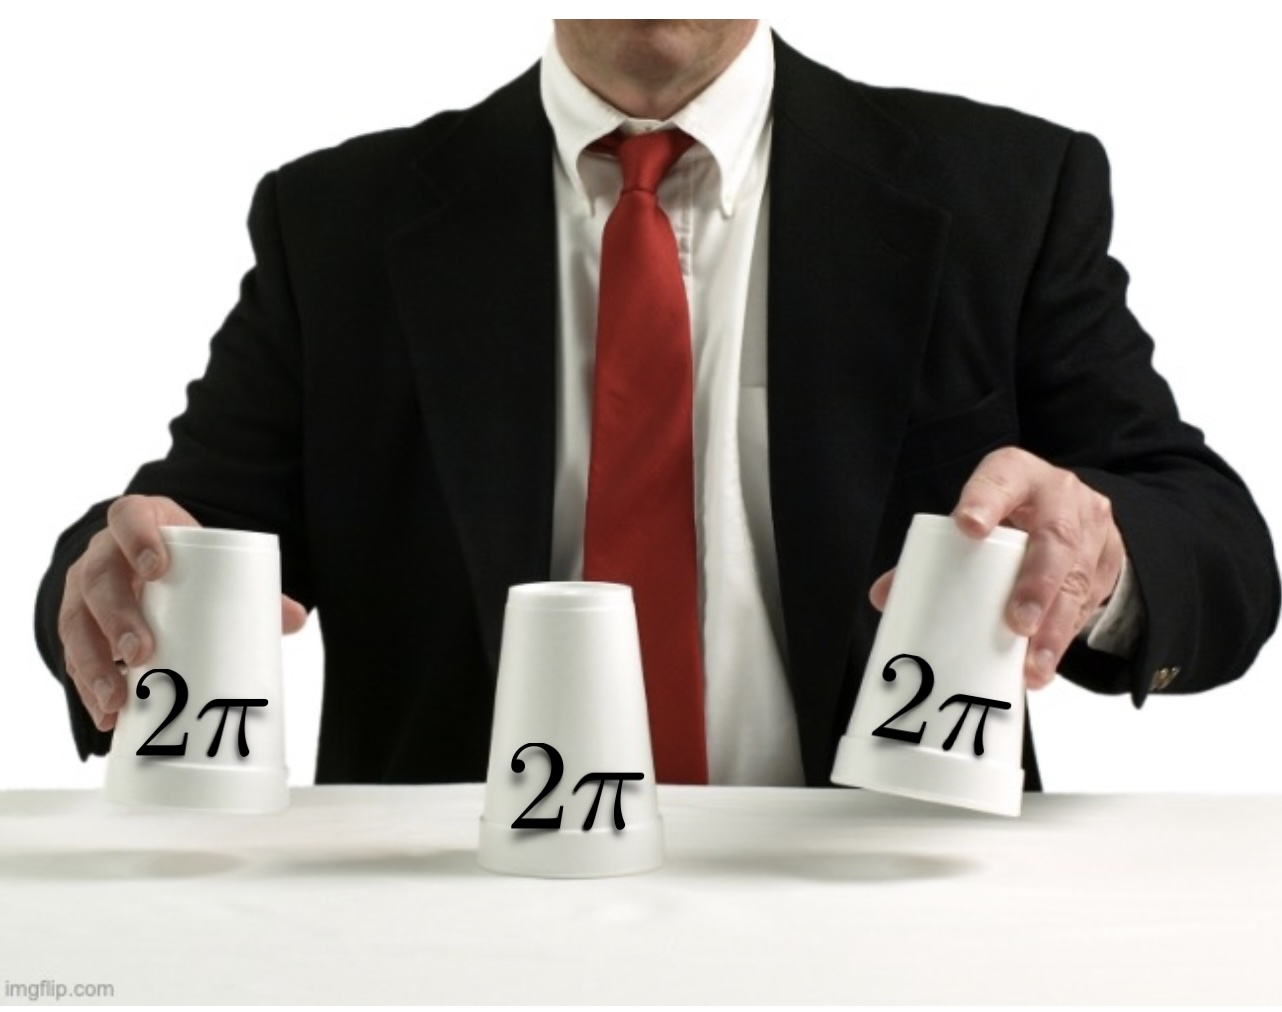
\includegraphics[width=\textwidth]{figures/2piShellGame.jpg}
    \captionsetup{font={scriptsize,sf}}
    \caption{How it feels keeping track of the $2\pi$ factors when comparing different Fourier conventions. Image adapted from \url{https://imgflip.com/i/8o9ed0}.}
    \label{fig:2pi:shell:game}
\end{marginfigure}
\begin{exercise}
Using the orthogonality of the complex exponentials, show that the coefficients $c_n$ in \eqref{eq:fourier:complex:series} are
\begin{align}
    c_n = \frac{1}{2\pi}\int_{-\pi}^\pi \D{\theta}\, f(\theta)\, e^{-in\theta} \ .
\end{align}
There's that famous factor of $2\pi$. Do not lose track of it.
\end{exercise}

Let us write this relationship explicitly in the form of an orthonormality relation:
\begin{align}
    \frac{1}{2\pi}
    \int_{-\pi}^\pi \D{\theta} \,
    % \frac
    {e^{in\theta}}
    % {\sqrt{2\pi}}
    % \frac
    {e^{-im\theta}}
    % {\sqrt{2\pi}}
    = 
    \begin{cases}
    1 &\text{if } n=m\\
    0 &\text{otherwise}
    \end{cases}
    \ .
\end{align}
\begin{example}[Freedom to choose bras and kets]
The expression above is indeed an orthonormality condition. The most natural assumption would be to define basis functions and dual functions
\begin{align}
    \ket{e_n} &\defeq \frac{e^{in\theta}}{\sqrt{2\pi}}
    &
    \bra{e_m} &\defeq 
    \int_{-\pi}^\pi \D{\theta} \, 
    \frac{e^{-in\theta}}{\sqrt{2\pi}}
    \Vtextvisiblespace[1em]{} \,
\end{align}
so that
\begin{align}
    \la e_m, e_n \ra 
    =
    \frac{1}{2\pi}
    \int_{-\pi}^\pi \D{\theta} \,
    % \frac
    {e^{in\theta}}
    % {\sqrt{2\pi}}
    % \frac
    {e^{-im\theta}}
    % {\sqrt{2\pi}}
     \ .
     \label{eq:complex:trig:function:inner:prod:even}
\end{align}
However, one could similarly define
\begin{align}
    \ket{e_n} &\defeq {e^{in\theta}}\ ,
\end{align} 
and posit that the $(2\pi)\inv$ in \eqref{eq:complex:trig:function:inner:prod:even} is part of the definition of the inner product. In this case the bra $\bra{e^m}$ has a funny asymmetric factor of $(2\pi)\inv$,
\begin{align}
    \bra{e^n} &\defeq \la e_n(\theta), \Vtextvisiblespace[1em]{} \ra 
    =
    \int_{-\pi}^\pi \D{\theta} \,
     \frac
    {e^{-in\theta}}
     {{2\pi}}
     \Vtextvisiblespace[1em]{} \,
    \ .
\end{align}
Here the empty space $\Vtextvisiblespace[1em]{}$ is meant to be a slot where you insert the vector (function) that the bra acts upon. From an aesthetic perspective, is is somewhat surprising that the typical convention in physics is to use the asymmetric convention.
\end{example}
The above example shows us that we \emph{may} write a set of basis functions \eqref{eq:complex:trig:function:inner:prod:even}---in fact, if you want to do this then you have the correct intuition for linear algebra. However, in physics it turns out to be convenient to chose a basis where we \emph{define} the inner product to have an extra factor of $(2\pi)^{-1}$ while keeping $\ket{e_n} = e^{in\theta}$. This will be because we are already used to \emph{angular} variables where this factor of $2\pi$ has a physical meaning: think of the difference between frequency and angular frequency. The latter has a factor of $(2\pi)^{-1}$ to give you  a \emph{per radian} measurement.





\section{From period to interval}

The variable $\theta \in [-\pi, \pi]$ might obscure our ultimate goal of representing functions over position. Let us replace the angular variable $\theta$ with a position variable over a range of distance $L$ centered around the origin, $x \in [-{L}/{2},L/2]$,
\begin{align}
    \theta = \alpha \frac{x}{L} = \frac{2\pi x}{L} \ .
\end{align}
The factor of $L$ denominator is necessary from dimensional analysis.\sidenote{$x$ has units of length whereas $\theta$ does not. Thus $\theta$ must be a ratio of $x$ to some other length.} The value of $\alpha = 2\pi$ is what is needed to map the interval $[-L/2,L/2]$ to the period $[-\pi,\pi]$. To avoid confusions about factors of $2\pi$, we leave it packaged as $\alpha$ for now. 

With these identifications, we now know that a real {function} $f(x)$ defined\sidenote{We are committing a small notational sin here. Technically we should call this a different function, $g(x) \equiv f(\alpha x/L)$. However, I hope it is clear that $f(x)$ differs from $f(\theta)$ by the rescaling of the argument.} over the interval $x\in[-L/2,L/2]$ may be written as
\begin{align}
    f(x) &= \sum_{n=-\infty}^\infty c^n e^{i\alpha n x/L} \ ,
    \label{eq:fourier:interval:complex}
\end{align}
where the Fourier coefficients are
\begin{align}
    c^n &= \frac{\alpha}{2\pi L} \int_{-\pi L/\alpha}^{\pi L/\alpha} \D{x}\; f(x)\, e^{-i\alpha n x/L} \ .
    \label{eq:fourier:interval:complex:coefficient}
\end{align}
One may insert $\alpha = 2\pi$ to simplify this, but for now we leave this factor separate to keep track of all of the $2\pi$ factors. The explicit factor of $(2\pi)\inv$ above is still the average over a period.


\begin{exercise}
Please appreciate that we are `unwinding' the circle here. The function $f(x)$ is formally defined over $x\in[-L/2,L/2]$, the region that we mapped to the circle. However, we can extend the definition to all of $x\in \mathbbm{R}$ if we assume that the real line just keeps winding around the circle. In this way, $f(x)$ with $x\in \mathbbm{R}$ is a periodic function that repeats itself with period $L$: $f(x) = f(x+L)$.
\end{exercise}

\noindent
The orthogonality condition over the ``physical'' (non-repeated) domain is 
\begin{align}
    \frac{\alpha}{2\pi L} \int_{-\pi L/\alpha}^{\pi L/\alpha} \D{x}\;
    e^{i\alpha n x/L}
    e^{-i\alpha m x/L}
    =
    \begin{cases}
    1 &\text{if } n=m\\
    0 &\text{otherwise} 
    \end{cases}
    \ .
\end{align}


\begin{exercise}[A silly sign convention]\label{ex:Fourier:using:Peskin:exponential:sign:convention}
Show that an alternative, equally valid definition of the Fourier series in \eqref{eq:fourier:interval:complex} is
\begin{align}
    f(x) = \sum_{n=-\infty}^\infty \tilde c^n e^{-i\alpha n x/L} \ .
    \label{eq:fourier:series:Peskin:convention}
\end{align}
This differs from \eqref{eq:fourier:interval:complex} by a minus sign in the argument of the exponential: $e^{i\alpha nx/L} \to e^{-i\alpha nx/L}$. The coefficients of this alternate Fourier series $\tilde c^n$ are different from those of the original series, $c^n$. However, this relationship is simple. Derive how $\tilde c^n$ and $c^n$ are related.

\textsc{Answer}: $\tilde c^n = c^{-n}$. The Fourier convention \eqref{eq:fourier:series:Peskin:convention} is what I use---it is what is standard in graduate textbooks in my field. This somewhat unusual minus sign can cause some head scratching if you are not aware of the alternative choices for how one may define the Fourier series.
\end{exercise}


\begin{example}[A silly prefactor convention.]\label{ex:Fourier:prefactor:convention}
There is nothing holy about writing the terms in \eqref{eq:fourier:interval:complex} as a coefficient times an exponential. Perhaps you would like to rescale the coefficient and compensate by rescaling the exponential? The following is an equivalent Fourier series:
\begin{align}
    f(x) = \sum_{n=-\infty}^\infty 
    \frac{c_n}{A} \, \left[A e^{i\alpha n x/L} \right] \ .
\end{align}
This is \emph{obviously} equivalent since the factors of $A$ simply cancel out and reproduce \eqref{eq:fourier:interval:complex}. What we demonstrate is that there is an arbitrary separation of prefactors between what we call the `basis functions' and the `coefficients.'\sidenotemark  In principle the rescaling factor $A$ could even be $n$-dependent. 
\end{example}\sidenotetext{You should worry that rescaling the basis functions spoils orthonormality. The trick here is that one must also redefine the definition of the inner product appropriately.}


\section{From integral to real line}
The discussion above gave a nice way of describing \emph{any} function over the interval $[-L/2, L/2]$ subject to the condition that $f(-L/2) = f(L/2)$. This condition is the periodic boundary condition coming from the original circle on which the function was understood to be defined.\sidenote{What is happening here is that the ``original'' space on which $f(\theta)$ is defined is a circle, $S^1$. This space is closed and has a periodic boundary condition.} We then said that we could extend the range of $x$ if we interpret this as continuing around the circle. When $L$ is very large, the periodic interval becomes so large that we find a representation of all functions on the interval $x\in (\infty, \infty)$. 

It behooves us to be a bit careful taking continuum limits, so let is take this limit carefully. In the sum over $n$ in \eqref{eq:fourier:interval:complex}, let us insert a \emph{trivial} factor of $\Delta n = 1$:
\begin{align}
    f(x) &= \sum_{n=-\infty}^\infty \Delta n\, c^n e^{i\alpha n x/L} \ .
    \label{eq:toward:fourier:transform:discrete:sum}
\end{align}
This factor is \emph{obviously} there and you can think of it as treating the right-hand side as a sum over a distribution.\sidenote{Think of a historgram. Each bin has a height that is proportional to some count. If you want the total number of counts in some interval, you are not actually summing all of the heights of the bin: you are summing the heights \emph{times their bin width}. Admittedly, often the bin width is one unit---but when the statistics are low, for example, you may want to have larger bins.} 

Now we want to take the $L\to \infty$ limit. If we do this na\"ively, it looks like the argument of the exponential immediately goes to zero. We realize, however, that we are being too quick: because the limits of the $n$ sum also go to $\pm \infty$, the product $nx$ for any $x\neq 0$ also goes to $\infty$. So it is better to think about ratios of quantities that each can go to $\pm\infty$. However, we want to keep the $x$-dependence explicit since the left-hand side is a function of $x$. This motivates us to define a variable with dimension of inverse length,
\begin{align}
    p \defeq \frac{\alpha n}{L} = \frac{2\pi n}{L} \in (-\infty,\infty) \ .
\end{align}
We deliberately label this with a character typically known to be \emph{momentum}, though formally this is a \emph{wave number}\index{wave number}.\sidenote{In natural units momenta and lengths have opposite dimension.} Most importantly, because $L\to\infty$, the ratio $n/L$ takes on any continuous value in $\mathbbm{R}$. We further identify 
\begin{align}
    \Delta p = \frac{\alpha \Delta n}{L} = 2\pi\frac{\Delta n}{L} \ .
\end{align}
In the $L\to\infty$ limit, this $\Delta p$ becomes infinitesimally small and we may write this as $\D{p}$. We thus find the continuum limit of the sum,
\begin{align}
    \sum_{n=-\infty}^\infty \Delta n &=
    \frac{L}{2\alpha} \int_{-\infty}^\infty \D{p} \ .
    \label{eq:toward:fourier:transform:sum:to:int}
\end{align}


The explicit factor of $L$ is a bit concerning since we know $L\to\infty$. However, we see that there is a compensating factor in $c^n$ in \eqref{eq:fourier:interval:complex:coefficient}. We proceed to write this Fourier coefficient as a function of the continuous variable $p$,
\begin{align}
    c^n \to c(p)
     &= \frac{\alpha}{2\pi L} \int_{-\infty}^{\infty} \D{x}\; f(x)\, e^{-ip x} 
     \equiv 
     \frac{\alpha}{2\pi L} \tilde{f}(p)
     \ .
    \label{eq:toward:fourier:transform:cn:to:cp}
\end{align}
In the last line we define the \textbf{Fourier transform}\index{Fourier transform} $\tilde{f}(p)$ of $f(x)$. 

A quick sanity check is in order. In both \eqref{eq:toward:fourier:transform:sum:to:int} and \eqref{eq:toward:fourier:transform:cn:to:cp} we have separately written the factor of $(2\pi)\inv$ coming from the original ``average over a period'' and the factor of $\alpha$ which came from mapping the period to a particular interval.\sidenote{$\alpha$ happens to equal $2\pi$.} What is significant is that in the Fourier representation of a function $f(x)$ defined over the entire real line, the factors of $\alpha$ cancel, but the ``average over a period'' does not. Plugging into \eqref{eq:toward:fourier:transform:discrete:sum} gives:
\begin{align}
    f(x) = \int_{-\infty}^\infty \frac{\D{p}}{2\pi}\; 
    % \left[\int_{-\infty}^\infty\D{x'}\, f(x') e^{-ipx'}\right] 
    \tilde f(p)\,
    e^{ipx} 
    \equiv 
    \int_{-\infty}^\infty \Dbar{p}\; 
    \tilde f(p)\,
    e^{ipx} 
    \ ,
\end{align}
where on the right-hand side we have defined the convenient notation\sidenote{I am surprised that this notation is not more standard.} $\Dbar{p} \equiv (2\pi)\inv \D{p}$. \eqref{eq:fourier:transform:convention} is called the \textbf{Fourier transform}\index{Fourier transform}. The definition of $\tilde f(p)$ is related to $f(x)$ by the \textbf{inverse Fourier transform}, \eqref{eq:toward:fourier:transform:cn:to:cp},
\begin{align}
    \tilde f(p) = 
    \int_{-\infty}^\infty \D{x}\, f(x)\, e^{-ipx} 
    \ .
\end{align}


\begin{newrule}[Fourier transform and its inverse]\label{rule:Fourier:transform:standard}
A function $f(x)$ of positions $x\in \mathbbm{R}$ may be equivalently encoded in a basis of plane waves and described by a function over momenta $p\in \mathbbm{R}$ as follows:
\begin{align}
    f(x) &= 
    \int_{-\infty}^\infty \Dbar{p}\; 
    \tilde f(p)\,
    e^{ipx} 
    \label{eq:fourier:transform:convention}
\\
    \tilde f(p) &= 
    \int_{-\infty}^\infty \D{x}\, f(x)\, e^{-ipx} 
    \ .
    \label{eq:fourier:inverse:transform:convention}
\end{align}
By dimensional analysis, the units of $p$ and $x$ are inverses of one another. In this notation, $\Dbar{p}\defeq \D{p}/2\pi$.
\end{newrule}

\section{Fourier Conventions}

% The Fourier transform \eqref{eq:fourier:transform:convention} and its inverse \eqref{eq:fourier:inverse:transform:convention}

The Fourier transform Rule~\ref{rule:Fourier:transform:standard} gives the momentum and position space representations of a function. However, there are signs and factors of $2\pi$ that can get shuffled around in different conventions, Figure~\ref{fig:2pi:shell:game}. One of the most annoying challenges in your physics life will be keeping track of signs and $2\pi$s across different conventions. Let us go over two such choices. These correspond to Exercise~\ref{ex:Fourier:using:Peskin:exponential:sign:convention} and Example~\ref{ex:Fourier:prefactor:convention}.\sidenote{Please review these before moving on.}

First, following Exercise~\ref{ex:Fourier:using:Peskin:exponential:sign:convention}, we observe that we may flip the sign of the momentum $p$ in the exponential:
\begin{align}
    f(x) &= 
    \int_{-\infty}^\infty \Dbar{p}\; 
    \tilde f(p)\,
    e^{-ipx} 
    \label{eq:fourier:transform:convention:sign}
\\
    \tilde f(p) &= 
    \int_{-\infty}^\infty \D{x}\, f(x)\, e^{+ipx} 
    \ .
    \label{eq:fourier:inverse:transform:convention:sign}
\end{align}
The coefficients $\tilde f(p)$ in this convention are numerically equivalent to the coefficients $\tilde f(-p)$ in the Rule~\ref{rule:Fourier:transform:standard} convention.

\begin{newrule}[Fourier conventions in this class]\label{rule:Fourier:transform:Flip}
While the derivation of the Fourier transform conventions in Rule~\ref{rule:Fourier:transform:standard} follow straightforwardly from our very reasonable discussion of the Fourier series, in \emph{this class} and in all of \emph{my work} I use the flipped-sign convention in \eqref{eq:fourier:transform:convention:sign} and\eqref{eq:fourier:inverse:transform:convention:sign} that is standard in particle physics.\sidenotemark 
\end{newrule}\sidenotetext{``\emph{My class, my rules.}''}

Secondly, one notices an asymmetry in the Fourier transform and its inverse: one has a factor of $(2\pi)\inv$ and the other does not.\sidenote{If you are a stickler for symmetry this probably really bothers you. I suspect this is another place where mathematicians are baffled why we would use such an odd notation.} You may even accuse me of trying to hide that factor of $2\pi$ by defining the $\Dbar{p}=\D{p}/(2\pi)$ notation. We emphasize that the existence of this $(2\pi)\inv$ is absolutely mathematically significant: it came from the fact that we have been averaging over an entire period. You might wonder if there is a way to more democratically distribute the $2\pi$ between $f(x)$ and $\tilde f(p)$. The answer is yes, as evidenced in Example~\ref{ex:Fourier:prefactor:convention}. We simply redefine $\tilde f(p)$ to absorb a $(2\pi)^{-1/2}$:
\begin{align}
    f(x) &= 
    \int_{-\infty}^\infty \frac{\D{p}}{\sqrt{2\pi}}\; 
    \tilde f(p)\,
    e^{ipx} 
    \label{eq:fourier:transform:convention:even:pi}
\\
    \tilde f(p) &= 
    \int_{-\infty}^\infty \frac{\D{x}}{\sqrt{2\pi}}\; 
    f(x)\, e^{-ipx} 
    \ .
    \label{eq:fourier:inverse:transform:convention:even:pi}
\end{align}
This notation is certainly more symmetric and perhaps easier to remember. However, physicists tend to use the asymmetric version where the $(2\pi)$ stays in one place.
\begin{example}
Why do physicists like this asymmetric notation? I suspect it connects to the way we teach angular frequency in introductory physics. At some point, most freshman physics students get a headache trying to figure out why there is both frequency and angular frequency: the two are related by a factor of $2\pi$. Well, my friend, \emph{this} is precisely that same factor of $2\pi$. It is the same $2\pi$ when we define \emph{wave number}. These factors of $2\pi$ show up in the volume of phase space in statistical mechanics and in quantum scattering. While it is ultimately a convention where we place them---the physical results are invariant---many of the physical quantities we care about in either position or momentum space have a straightforward interpretation with the $2\pi$ in `one place.'
\end{example}

\section{\texorpdfstring{Rediscovering $\delta$}{Rediscovering delta}}

There is a consistency condition for whatever conventions you use for the Fourier transform: if you do the Fourier transform and then the inverse Fourier transform, then you had better return to the original function. Let us see this in action using the Fourier conventions in Rule~\ref{rule:Fourier:transform:Flip}. We start by expressing $f(x)$ in terms of its Fourier modes $\tilde f(p)$, \eqref{eq:fourier:transform:convention:sign}
\begin{align}
    f(x) &= 
    \int_{-\infty}^\infty \Dbar{p}\; 
    \tilde f(p)\,
    e^{-ipx} 
    \ .
\end{align}
Next, insert the expression for $\tilde f(p)$ in terms of the original function \eqref{eq:fourier:inverse:transform:convention:sign},
\begin{align}
f(x) &= 
    \int_{-\infty}^\infty \Dbar{p}\; 
    % \tilde f(p)\,
    \left[
     \int_{-\infty}^\infty \D{y}\, f(y)\, e^{ipy} 
    \right]
    e^{-ipx} 
    \\
    &=
    \int_{-\infty}^\infty \D{y}\; f(y)
    \int_{-\infty}^\infty \Dbar{p}\, \, e^{-ip(x-y)} 
    \ ,
    \label{eq:fourier:transform:delta:function:int1}
\end{align}
where we had to use a different dummy\sidenote{We say `dummy variable' in the sense of a dummy index. The expression itself has no actual $y$ dependence because the dummy variable $y$ is integrated over.} position variable $y$ so as to not confuse it with the not-dummy variable $x$. 

Take a good look at \eqref{eq:fourier:transform:delta:function:int1}. The $\Dbar{p}$ integral evaluates to some function\sidenote{Technically a \emph{distribution}.} over $y$ that, when integrated with $\D{y}\, f(y)$, produces $f(x)$. There is a function that does this: the Dirac $\delta$-function. We have found the Fourier representation of the $\delta$ function:
\begin{align}
    \delta(x-y) = \int \Dbar{p}\, e^{-ip(x-y)} \ .
    \label{eq:fourier:representation:of:Dirac:delta}
\end{align}
Do not forget that $\Dbar{p} = \D{p}/(2\pi)$.

\begin{exercise}
Show that the manipulations in this section give the same result, \eqref{eq:fourier:representation:of:Dirac:delta}, even if we were using the Rule~\ref{rule:Fourier:transform:standard} Fourier conventions. Show the same for the `democratic' Fourier convention in \eqref{eq:fourier:transform:convention:even:pi} and \eqref{eq:fourier:inverse:transform:convention:even:pi}.

You should appreciate that the $(2\pi)$ is \emph{really there} and not some convention-dependent artifact. Comment on the sign of the argument of $\delta(x)$---does it matter? Does the sign of $p$ in the exponential of \eqref{eq:fourier:representation:of:Dirac:delta} matter?
\end{exercise}

\begin{exercise}
Show in one line that \eqref{eq:fourier:representation:of:Dirac:delta} is equivalent to
\begin{align}
    \delta(x) = \int_{-\infty}^\infty \D{q}\; e^{2\pi i xq} \ ,
\end{align}
which is another common integral representation of the $\delta$-function.
\end{exercise}

\section{Momentum Space and Its Cousins}

What does the Fourier transform buy us? The power of the Fourier transform is that we are able to represent a function in terms of a sum (integral) over momentum eigenstates, $e^{-ipx}$. In turn, the magic of these states is that they are \emph{eigenstates} of the derivative operator:
\begin{align}
    \frac{\D{}}{\D{x}} e^{-ipx} = (-ip) e^{-ipx} \ .
\end{align}
\begin{example}
Note that the eigenvalue of $\D{}/\D{x}$ is not real. This is because the single derivative is not a Hermitian operator. A more proper statement is that a momentum eigenstate is an eigenstate of the Laplacian, $(\D{}/\D{x})^2$ with eigenvalue $-p^2$.
\end{example}
\begin{exercise}
In more than one dimension, the momentum eigenstates are $e^{-i p\cdot x}$ where $p\cdot x = p_\mu x^\mu$. Show that these satisfy
\begin{align}
    \frac{\partial}{\partial x^\mu} e^{-ip\cdot x}
    &= (-ip_\mu) e^{-ip\cdot x} \ .
\end{align}
This is a simple extension of the single dimensional case, but please make sure you follow both the presence of the $\mu$ index and its height on each side of the equation.
\end{exercise}

\paragraph{Solving differential equations}
Eigenstates of the derivative are \emph{especially} useful in physics because, as we motivated in \bigidearef{}~\ref{idea:causality:and:derivatives}, the laws of physics are written in terms of derivatives.\sidenote{Recall that one way to see this is a requirement of causality.} In fact, often times we have equations of the form 
\begin{align}
    (\text{differential operator}) f(x) &= s(x) \ ,
\end{align}
where we want to determine some state $f(x)$ as a function of some known source $s(x)$. The differential operator is some polynomial of derivatives,\sidenote{I am writing derivatives as partial derivatives in anticipation of $x$ being multidimensional in many cases.} $P(\partial)$. For example, the Laplacian/d'Alembertian is
\begin{align}
    P(\partial) = \partial_\mu \partial^\mu = \frac{\partial}{\partial x^\mu}\frac{\partial}{\partial x_\mu} \ .
\end{align}
When we write $f(x)$ as a Fourier transform, each term in the integral/sum contains simple $x$-dependence: $e^{-ip\cdot x}$. Then the action of $P(\partial)$ becomes multiplication by a polynomial in $p$:
\begin{align}
    P(\partial) e^{-ip\cdot x}
    = 
    P(-ip) e^{-ip\cdot x} \ .
\end{align}
\begin{exercise}
Confirm the above equation. 
\end{exercise}
Further, this means that \emph{inverting} the equation becomes easy---at least writing down a closed form integral:
\begin{align}
    P(\partial) 
    \int \DDbar{d}{p}\, \tilde f(p)
    e^{-ip\cdot x}
    =
    \int \DDbar{d}{p}\, \tilde f(p) P(-ip) 
    e^{-ip\cdot x}
    = 
    \int \DDbar{d}{p}\, \tilde s(p)
    e^{-ip\cdot x} \ .
\end{align}
Then we may identify the coefficients of independent $e^{-ip\cdot x}$ modes for each $p$:
\begin{align}
    \tilde f(p) = \frac{\tilde s(p)}{P(-ip)} \ .
\end{align}
Specifying each of the Fourier components of a function $f(x)$ is equivalent to specifying the entire function. Thus one has solved the differential equation.\sidenote{One has solved it in momentum space, but one still has to perform an inverse Fourier transform to write it in position space, so there's still an integral to be done. There is definite progress, though: often this integral can be approximated, numerically if need be.}





\paragraph{Special functions} The general procedure here is something that shows up over and over in mathematical physics:
\begin{bigidea}[Why do some functions have names?]\label{rule:special:functions}
There is a surprisingly small number of `really important differential operators' that show up over and over in physics. These tend to be cousins of the Laplacian. These operators have some natural basis of eigenfunctions that are the \emph{correct} basis to use to solve any differential equation in a straightforward way. Because these eigenfunctions are so common in physics, we end up giving them names. You may have heard of Bessel functions, Legendre polynomials, spherical harmonics, Airy functions, and so forth. If an exotic-looking class of functions has a name, it is probably the eigenfunction of some significant differential operator. So when you meet these functions, do not think that you have met some weird new species: ask `what operator is this an eigenfunction for'? Once you understand these functions as an orthonormal basis, you have no reason to fear or be puzzled by them. 
\end{bigidea}
Please keep this organizing principle in mind every time you meet a new family of special functions. It is a `unification' of the general approach to all sorts of physics problems---especially the ones that show up in first-year graduate courses. 


\begin{exercise}[Why are there so few differential operators?]\label{ex:few:differential:ops}
The observation in \bigidearef{}~\ref{rule:special:functions} assumes that there are only a few `really important differential operators' in physics. In fact, these are essentially the Laplacian (second derivative) written in different coordinate systems. Why is this? 

One way to argue is to assume that the laws of physics are derived from an action principle: there exists some scalar function  $S=\int \D{t}\, L[\cdots]$ that depends on the dynamical variables (`states') of your physical theory. This is true in all of your physics courses.  This scalar function contains derivatives, as per \bigidearef{}~\ref{idea:causality:and:derivatives}. Argue that the second derivative is the most significant term.

Argue that the first derivative does not typically contribute because then there is no natural way for $S$ or $L$ to be a scalar function. Argue that third and higher derivatives do not typically contribute from dimensional analysis. This latter point comes from recognizing that the action and the dynamical fields carry some units. The derivative, too carries units. Terms with more derivatives must then have these units compensated by some scale. In a physical theory, scales that are `put in by hand' represent \emph{microphysics}: the underlying dynamics that lie \emph{beyond} the present theory. For example, a theory of light passing through the atmosphere may have the typical size of a nitrogen molecule as its microscopic scale. At length scales smaller than this, the interactions of photons with the molecule cannot be described by the typical Rayleigh theory that explains why the sky is blue.

This exercise has a conceptually simple answer, but it draws on a rather sophisticated understanding of physics---it is rather subtle if you have not thought about this before. Feel free to ask about it in class. 
\end{exercise}








\begin{subappendices}
\section{A general Fourier transform}

There are two choices one can make when defining a Fourier transform convention\footnote{This appendix draws from an excellent discussion at \url{https://physics.stackexchange.com/a/308248}}; we parameterize these choices by real numbers $a$ and $b$. The Fourier transform $\tilde f(\omega)$ of a function $f(t)$ is
\begin{align}
  \tilde f(\omega)
  &= 
  \sqrt{\frac{|b|}{(2\pi)^{1-a}}}
  \int_{-\infty}^\infty \D{t}\, e^{ib\omega t} f(t) \ .
\end{align}
We see that $a$ tells us about the $(2\pi)$ factors and $b$ tells us about the argument of the basis function $e^{ib\omega t}$. With this basis, the inverse Fourier transform is 
\begin{align}
  f(t)&=
  \sqrt{\frac{|b|}{(2\pi)^{1+a}}}
  \int_{-\infty}^\infty \D{\omega}\, e^{-ib\omega t} f(\omega) \ .
\end{align}

One may check that the inverse Fourier transform of a Fourier transform gives the original function:
\begin{align}
  \tilde{\tilde f} &=
  \frac{|b|}{2\pi}
  \int_{-\infty}^\infty \D{\omega}\, e^{-ib\omega t}
  \int_{-\infty}^{\infty}
  ds\, e^{ib\omega s} f(s)
  \\
  &= 
  \frac{|b|}{2\pi}
  \int ds\, f(z) \int \D{\omega} \, e^{ib\omega(s-t)}
  \\
  &= \int \D{s}\, \delta(s-t) f(s) \ ,
\end{align}
where we have used $\int \D{\xi} \exp(2\pi i x\xi) = \delta(x)$. 

\section{Our Conventions}
\label{app:Fourier}

The convention that we will choose for the \emph{time}--\emph{frequency} [inverse] Fourier transform is
\begin{align}
  f(t) &= \int_{-\infty}^{\infty} \Dbar\omega
  \; e^{-i\omega t} \tilde f(\omega)
  &
  \Dbar\omega &\equiv\frac{d\omega}{2\pi} \ .
\end{align}
This corresponds to $a=b=1$. The corresponding transform for the frequency-domain function is
\begin{align}
  \tilde f(\omega) &= 
  % \frac{1}{2\pi}
  \int_{-\infty}^\infty \D{t}\, e^{i\omega t} f(t) \ .
  \label{eq:inverse:fourier:convention}
\end{align}

\section{Higher Dimensions}

All of this generalizes to higher dimensions: you simply Fourier transform each dimension. In fact, one is free to use a different Fourier transform convention for each direction. We can use this freedom to pick a convention that `automatically' fits our conventions for spacetime. In particular, given a four-vector $x=(t,\vec{x})$ and its conjugate four-momentum $p=(\omega, \vec{k})$, one may choose to Fourier transform as follows: 
\begin{align}
  f(x) &= \int \Dbar\omega \DDbar{3}{\vec{k}}\; 
  e^{-i(\omega t-\vec{k}\cdot\vec{x})} \tilde f(p)
  \ .
\end{align}
With this convention, the basis function is simply
\begin{align}
  e^{-i(\omega t-\vec{k}\cdot\vec{x})} 
  = e^{-ip\cdot x} \ , 
\end{align}
where $p\cdot x$ is the usual Minkowski dot product, $p_\mu x^\mu$. This makes it clear that the basis function is Lorentz invariant. The Fourier transform would still respect the spacetime symmetries even if we had not chosen a convenient notation---it just wouldn't be as simple to see.



\begin{example}
\textbf{Statistical Mechanics.} One motivation for our Fourier convention is statistical mechanics. One formulation of classical statistical mechanics is to assume that phase space is discrete: a particle has momentum $\vec{p}$ whose components take integer multiples of some unit momentum, $h$. Assuming that the particle has $g$ internal degrees of freedom (e.g.~$g=2$ for a particle that can be spin-up or spin-down), then the density of states is $g/h^{3}$. Quite remarkably in the history of physics, the value of $h$ can be identified with Planck's constant in quantum mechanics. In natural units we take $\hbar = h/(2\pi)\equiv 1$, so the phase space density is $g/(2\pi)^3$. For a particle with a phase space distribution function $f(\vec{x},\vec{p})$, this means that the number density of particles is
\begin{align}
  n = g\int \DDbar{3}{\vec{p}} \, f(\vec{p}) \ .
\end{align}
We see that it is convenient to take a convention where every $\D{p}$ comes with a $(2\pi)^{-1}$.
\end{example}

\begin{exercise}\textbf{Lorentz-Invariant Phase Space.}
% See also https://physics.stackexchange.com/questions/141724/why-is-there-1-2-pi-in-int-fracdp2-pip-rangle-langle-p (
% Josh's response)
In relativistic systems, the energy and the momenta are related by $E^2 = \vec{p}^2 + m^2$. We are, of course, using natural units where $c=1$. The phase space integral over $\DDbar{3}{\vec{p}}$ is thus also an integral over the energy. In order to enforce the relativistic relation, the full phase space density is usually written as $\DDbar{4}{p}\, (2\pi)\,\delta(E^2-p^2-m^2)\,\Theta(E)$. The Heaviside step function $\Theta(E)$ is one when $E\geq 0$ and zero otherwise; it ensure that the outgoing energies are positive. Show that integrating over the $\delta$-function gives
\begin{align}
  \int \DDbar{4}{p}\, \delta(E^2-p^2-m^2) &= 
  \int \frac{\DDbar{3}{\vec{p}}}{2E(p)}
  &
  E(p) \equiv \sqrt{p^2 + m^2} \ .
\end{align}
\textsc{Hint}: use the relation
\begin{align}
    \delta(f(x)) &= \sum_{x_i} \frac{\delta(x-x_i)}{\left|\D{f}(x_i)/\D{x}\right|}
\end{align}
where the sum is over the root of $f(x)$, that is: one sums over the $x_i$ such that $f(x_i)=0$. The $\Theta$ function ensures that only one such root contributes.
\end{exercise}

\end{subappendices}
